\begin{savequote}[0.55\linewidth]
	\begin{fancyquote}
		Each discovery made by an investigator in a basic research
		laboratory has much larger implications today. The sum of the work in basic
		biology represents a rapidly expanding tool kit for engineers and inventors to
		use to construct items of value to society.
	\end{fancyquote}
	\qauthor{David Baltimore in \emph{How Biology Became an Information Science}, 2001~\autocite{Baltimore:2001}}
\end{savequote}
\chapter{Introduction}\label{ch:introduction}

This thesis aims to detail the design and implementation of a
neuron morphology extraction system. This system is the result of
converting the existing ORION 3~\autocite{ORION_Santamaria-Pang2015} system from
MATLAB~\autocite{MATLAB:2013a} code to native C/C++ code.
This conversion process requires an analysis of the existing code
to understand its structure and create a plan for replicating the
same functionality in the in the new system.

This software project can be categorised as a \emph{rewrite}; that
is, a replication of an existing software system without
reusing the existing code. In software engineering, the consensus
on rewriting software from scratch is that it is difficult and
that teams should avoid rewrites~\autocite{Software-rewrites:Spolsky:2000}. This view
arises because there are several challenges and risks associated
with rewriting large systems.
% reasons why rewrites fail
\begin{itemize*}[label={}]
\item Rewrites often take a long time and instead of adding
	features, development time is spent on redesign and
	reimplementation of old features.
\item In addition, all the institutional knowledge that came from
	years of bug fixes is often lost with a rewrite.
\item Rewrites are often expensive in terms of time and effort and
	are not known to payoff as much as product owners wish.
\end{itemize*}
% refactoring over rewriting
As such, it is preferable to work on slowly refactoring the code
rather than a complete rewrite. Refactoring is a process where
instead of throwing away the existing system, the development
proceeds by making small, incremental changes over an extended
period in order to avoid getting the software into a broken state,
while steadily improving the readability and reusability of the
software.

\section{Motivation}
%  [ Discussion of the application area and context of the
%    project. ]

% understand the goals of the project by talking about the background
In order to understand why this project is being undertaken, it is
important to understand why a rewrite is necessary as opposed to refactoring
the existing codebase. Both options require an analysis of the project
deliverables, that is, a concrete set of goals that will direct the project
development. These deliverables can be classified as either scientific or
engineering deliverables. Scientific deliverables are motivated by goals that
advance the state of scientific knowledge while engineering deliverables focus
on specific technical aspects of the project that make future project
maintenance and growth possible. This section will only cover the scientific
deliverables while engineering deliverables are covered in Section~\ref{sec:deliverables}.

The \emph{primary scientific deliverable} of this thesis is a system for
neuron reconstruction. This system is designed with the principles of open
science in mind so that it is usable by biologists to study
neuroanatomy. Section~\ref{subsec:open-science} contains further
discussion on open-science and how this project achieves this
goal.

The \emph{secondary scientific deliverable} is to make this system
compatible with existing tools for image analysis so that it can
be compared against other methods as part of the BigNeuron
project. The role of BigNeuron in neuroscience research is covered
in Section~\ref{subsec:bigneuron}.

The following sections contain an overview of the context of this project
first within the general context of scientific software (Section~\ref{subsec:sci-soft})
and finally narrow down its role relative to the specific context
of neuron reconstruction (Section~\ref{subsec:neuron-tracing}).

\subsection{Scientific software}\label{subsec:sci-soft}
{ % how software has become important in experimental science
	Quantitative methods are an essential part of scientific research. The
	experimental sciences depend on the dissemination of the methods used for each
	study so that it is clear how results are obtained and analysed.
	With the rapid increase in computing power, storage, and availability,
	it has become easier to collect and process larger and more complex datasets
	using sophisticated methods and this has made software and
	software development an important part of all experimental
	fields~\autocite{SSI:hettrick_2014_14809}.
	To produce reproducible results, some common approaches to this change are
	to publish either a description of the algorithm or refer to software
	that can be obtained separately (either in binary or source code form).
}

Despite these approaches, there are still several challenges to a successfully
reproducing a published method.
{ % problems with a textual description
	A textual description of an algorithm is rarely a complete description of
	how an algorithm is implemented. Sophisticated methods often have tiny details
	that are mistakenly left out which may be essential for the rest of the
	processing. One specific area where this occurs often is
	in data preprocessing and annotation stages which can
	involve human interaction and, as such, some assumptions
	may not be written down.
}
{ % problems with software distribution
	Referencing readily available software packages gives
	other researchers direct access to the original method
	used. However, even here, there can be problems.
	Even before running the software, it is important to
	ensure that the
	software is available years later. This means not only the software itself, but
	all its dependencies. This can quickly become complicated as technology
	advances: changes in the Application Programming Interface (API) or Application
	Binary Interface (ABI) can cause incompatibility issues for both
	software distributed in source form or
	binary form. Both source code and binary software can have
	dependencies on platforms (e.g., operating systems,
	runtimes, computer architecture, etc.) and licensing of
	components that can hinder others from using the software.
}

{ % backwards compatibility and digital preservation
	Even more precarious is when a dependency used by the
	software no longer behaves the same way as it did in
	previous versions. This can lead to software that appears
	to run, but gives unintended results. Maintaining
	backwards compatibility for software is difficult since
	there are many parts to a non-trivial software system.
	% Dependency hell
	Resolving the exact versions of libraries and toolchains
	needed to build and run can be frustrating and is commonly
	known as \emph{dependency hell}. This problem can become
	daunting when dealing with multiple platforms and many
	libraries. As newer versions of these libraries are
	released, the maintenance stage of the \emph{systems
	development life cycle} becomes more important (see Figure~\ref{fig:sdlc}).
	Unmaintained software is prone to what is known as
	\emph{bit rot} --- that is, the process through which
	software that was working no longer works due to changes
	in the surrounding software ecosystem.
	There has been some work to prevent bit rot by recording a
	static copy of the software environment, but digital
	preservation (comprising both computing machinery and
	software) is in its infancy and has not caught up to that
	of paper-based materials~\cite{Owens2013,Thain2015,Meng2015}.
}
\begin{figure}
\centering
%% Diagram of systems development life cycle
%%
%% Base TikZ taken from <http://www.texample.net/tikz/examples/circular-arrows-text/>.
%%
%% See also: sdlc-preamble.tex
\usetikzlibrary{decorations.text}
\newcommand*{\mytextstyle}{\sffamily\normalsize\bfseries\color{black!85}}
\newcommand{\arcarrow}[8]{%
% inner radius, middle radius, outer radius, start angle,
% end angle, tip protusion angle, options, text
  \pgfmathsetmacro{\rin}{#1}
  \pgfmathsetmacro{\rmid}{#2}
  \pgfmathsetmacro{\rout}{#3}
  \pgfmathsetmacro{\astart}{#4}
  \pgfmathsetmacro{\aend}{#5}
  \pgfmathsetmacro{\atip}{#6}
  \fill[#7] (\astart:\rin) arc (\astart:\aend:\rin)
       -- (\aend+\atip:\rmid) -- (\aend:\rout) arc (\aend:\astart:\rout)
       -- (\astart+\atip:\rmid) -- cycle;
  \path[font = \sffamily, decoration = {text along path, text = {|\mytextstyle|#8},
    text align = {align = center}, raise = -0.5ex}, decorate]
    (\astart+\atip:\rmid) arc (\astart+\atip:\aend+\atip:\rmid);
}

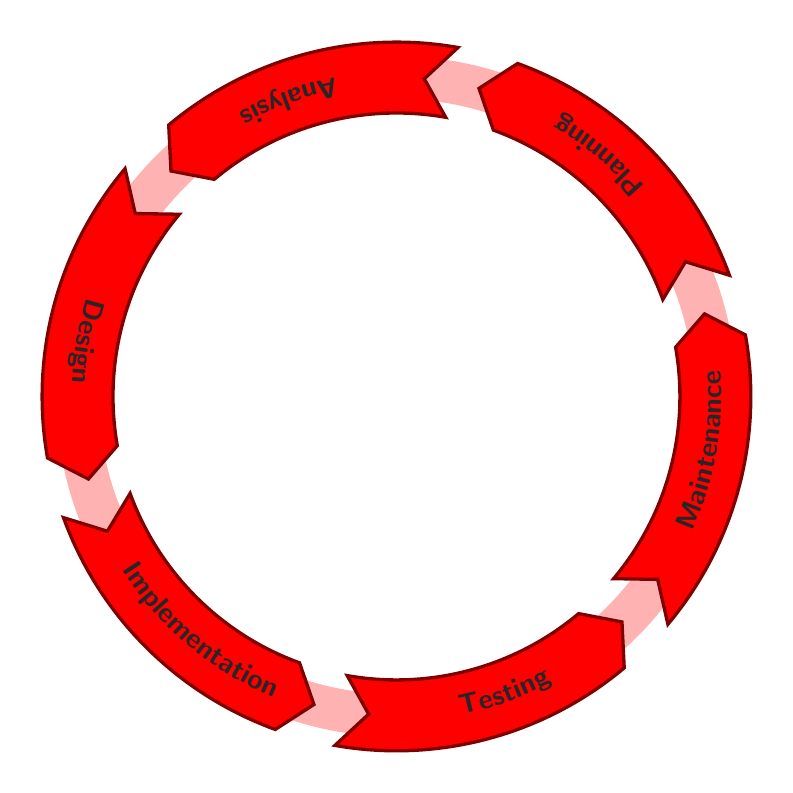
\begin{tikzpicture}[scale=0.9]
  \fill[even odd rule,red!30] circle (4.8) circle (4.2);
  \foreach \x/\text in {0/Planning,1/Analysis,2/Design,3/Implementation,4/Testing,5/Maintenance} {
    \arcarrow{4}{4.5}{5}{\x*60+20}{\x*60+70}{5}{red,draw = red!50!black, very thick}{\text}
  }
\end{tikzpicture}

\caption{Systems development life cycle}\label{fig:sdlc}
% TODO describe the systems development life cycle
\end{figure}


\subsection{Open science and scientific software engineering}\label{subsec:open-science}

As science becomes more oriented towards using computational
tools, the ideals of reproducibility and statistical hypothesis
testing become more difficult to achieve. In recent years, there
has been a push by researchers to incorporate \emph{open science}
practices in their work. One prominent advocate for open science
defines it as
\begin{quote}
	\begin{fancyquote}
	Open science is the idea that scientific knowledge of all kinds
	should be openly shared as early as is practical in the discovery
	process.
	\end{fancyquote}
	\qauthor{Michael Nielsen\footnote{http://michaelnielsen.org/blog/open-science-2/}} % TODO add more info about quote
\end{quote}

% Principles of open science <http://openscienceasap.org/open-science/>
%
%   Open Methodology
%   Open Source
%   Open Data
%   Open Access
%   Open Peer Review
%   Open Educational Resources

% <https://github.com/openscienceASAP/open-science-sticker>


% TODO
Software Carpentry, Software Sustainability Institute


\subsection{Open neuroscience}
% TODO
Biology and neuroscience in particular have been using more
quantitative imaging tools: patch clamp, EEG, fMRI, fluorescent
microscopy ... need to measure what is being looked at ... perform
statistical analysis across samples

% TODO
Allen Institute for Brain Science,
Big Brain project,
Big Neuron
NITRC
Neuinfo  Framework
Neuromorpho
EyeWire
Knossos / Brainflight
VirtualFlyBrain
~\autocite{NeuroDebian:Halchenko:2012}

\subsection{BigNeuron}\label{subsec:bigneuron}

{ % what is Vaa3D
	The secondary deliverable is to make the system compatible
	with the Vaa3D biomedical imaging toolkit~\autocite{Vaa3D:site:2015,Vaa3D:Peng:2010,Vaa3D:Peng:2014}.
	This toolkit allows biologists to visualise and analyse
	biomedical imaging datasets. It can be extended through
	the development of plugins. This allows algorithm
	developers to make their both their interactive and
	non-interactive methods for image analysis available
	for biologists to use without having to switch between
	multiple programs for processing and visualising data.
}

% explain comparing algorithms and DIADEM Challenge
Creating an image analysis tool that can be easily integrated into
other systems allows others to reproduce the results in order to
compare with ground truth data and other algorithms. There
has been an attempt at comparing neuron morphology extraction
algorithms in the past under the DIADEM Challenge which
contributed datasets and a metric for comparing the neuron
tracings from algorithms against tracings from gold standard
segmentations~\autocite{DIADEM&Beyond:Liu:2011,DIADEM-dataset:Brown:2011,DIADEM-metric-Gillette2011}.
The DIADEM Challenge used 6 datasets from different neuroscience
institutions in order to have a diversity in terms of source of
the neurons (i.e., from different species and structures from
different brain regions) and in terms of the laboratory protocols
(i.e., different labelling and microscopy techniques).

The DIADEM Challenge was successful in raising awareness of the
problem of neuron reconstruction and several new 3D reconstruction
methods and metrics have been proposed after the end of the DIADEM
Challenge (see Section~\ref{subsec:neuron-tracing}).  However, the
lack of larger public datasets, standardised metrics, and readily
available algorithms have made it difficult to compare new methods
for neuron reconstruction.

% explain BigNeuron
To solve this problem, an open-science project called
BigNeuron~\autocite{BigNeuron:Peng:2015,DIADEM2BigNeuron:Peng:2015}
continues where the DIADEM Challenge left off. Instead of
comparing the output on a few datasets as in the DIADEM Challenge,
BigNeuron aims to enable high-throughput analysis of neuron
microscopy stacks using multiple methods contributed from various
algorithm developers. By standardising on the Vaa3D platform, this
precludes differences between how each method handles data which
means that all the algorithms can be bench-tested at once without
a need for translating data between formats.

However, since the Vaa3D is written in C++, incorporating plugin
code written in non-native languages poses a problem. For this
reason, the BigNeuron project organisers recommend that all
algorithms that are submitted be in C or C++. From the BigNeuron
FAQ~\autocite{BigNeuron:FAQ:2015}
\begin{quote}
	\begin{fancyquote}
		{Q3. \bfseries How can I incorporate code written in Matlab, Java, Python or another language other than C/C++?}

		A. BigNeuron is a very large scale project, and enforcing a
		unified API is critical to ensure fair comparison for any pre-defined
		assessment. We thus discourage usage of Matlab, Java, Python or other
		programming languages besides C/C++ for this bench
		testing.
	\end{fancyquote}
\end{quote}

\subsection{Engineering motivation}

In addition, a rewrite allows for more thorough
design and testing which is necessary to verify that the code
behaves as expected and will continue to do so in the future.

\section{Literature review}

\subsection{Neuron reconstruction and tracing}\label{subsec:neuron-tracing}

~\autocite{Duke-Southampton-archive:Cannon:1998,DIADEM-dataset:Brown:2011,NeuroMorphVariability:Parekh:2015}

~\autocite{DIADEM&Beyond:Liu:2011,NeuroMorphTrends:Halavi:2012,NeuroTracePerspect:Meijering:2010}

Post-DIADEM
~\autocite{Bauer2010,MIA-anisotropic-path-searching-Xie2011,MICCAI-anisotropic-path-searching-Xie2010,
Jeong2015,Luo2015,De2015,Gulyanon2015,ORION_Santamaria-Pang2015,Mukherjee2014,Hernandez-Herrera2014,Basu2014,Xiao2013,Jimenez2013,Basu2013,Mukherjee2013,Hernandez-Herrera2013,Ming2013,Lee2012,Czarnecki2012}

metrics~\autocite{Mayerich2011,Mayerich2012,btmorph-Torben-Nielsen2014,Costa2014,Gillette2015}

\begin{enumerate}[label=(\roman*)]
\item to evaluate the MATLAB codebase of ORION 3 and determine how to structure the new codebase
\item integrate the
\end{enumerate}

% TODO
%
% - refactoring and conversion of code
% - Open science
% - bioinformatics

\section{Survey of libraries used}

% - cite the architecture of open-source applications
% - ITK
% - VTK

